\section{\texorpdfstring{$B$}{B} meson production in proton-proton collisions}
\label{sec:B_mesons}

A proton-proton collision ($pp$-collision) is the interaction between two high energetic protons through the strong force.
The exchange of gluons between those protons initiates the production of multiple particles. 
Important at LHCb are primarily $pp$-collisions in which $b$ hadrons are produced.
The dominant process for $b$ hadron production is the fusion of two gluons into one gluon, which then decays into a $b\bar{b}$ pair.
These $b$ quarks then hadronize by combining with other quarks that emerge from the vacuum in pairs.
This then also produces fragmentation particles through further hadronization of the unpaired quarks.

A frequent goal at LHCb is to analyse $pp$-collisions for $B$ meson candidates, often called the signal $B$.
$B$ mesons are composed of one $b$~quark and one of the $u/d/c/s$ quarks.
Relevant for this thesis are the uncharged $B$~mesons
\begin{align*}
    B^0 &= \bar{b}d \, , & \bar{B}^0 &= b\bar{d} \, , & B_s^0 &= \bar{b}s \, , & \bar{B}_s^0 &= b\bar{s} \, .
\end{align*}

The algorithm developed in this thesis distinguishes $B_d$ mesons ($B^0$ and $\bar{B}^0$) from $B_s$ mesons ($B_s^0$ and $\bar{B}_s^0$).
An example schematic of a $pp$-collision containing a $B$ meson is shown in \autoref{fig:ft_scheme}. 
This schematic excludes particles which are unassociated with the signal $B$ that are contained in the underlying event.

\begin{figure}
    \centering
    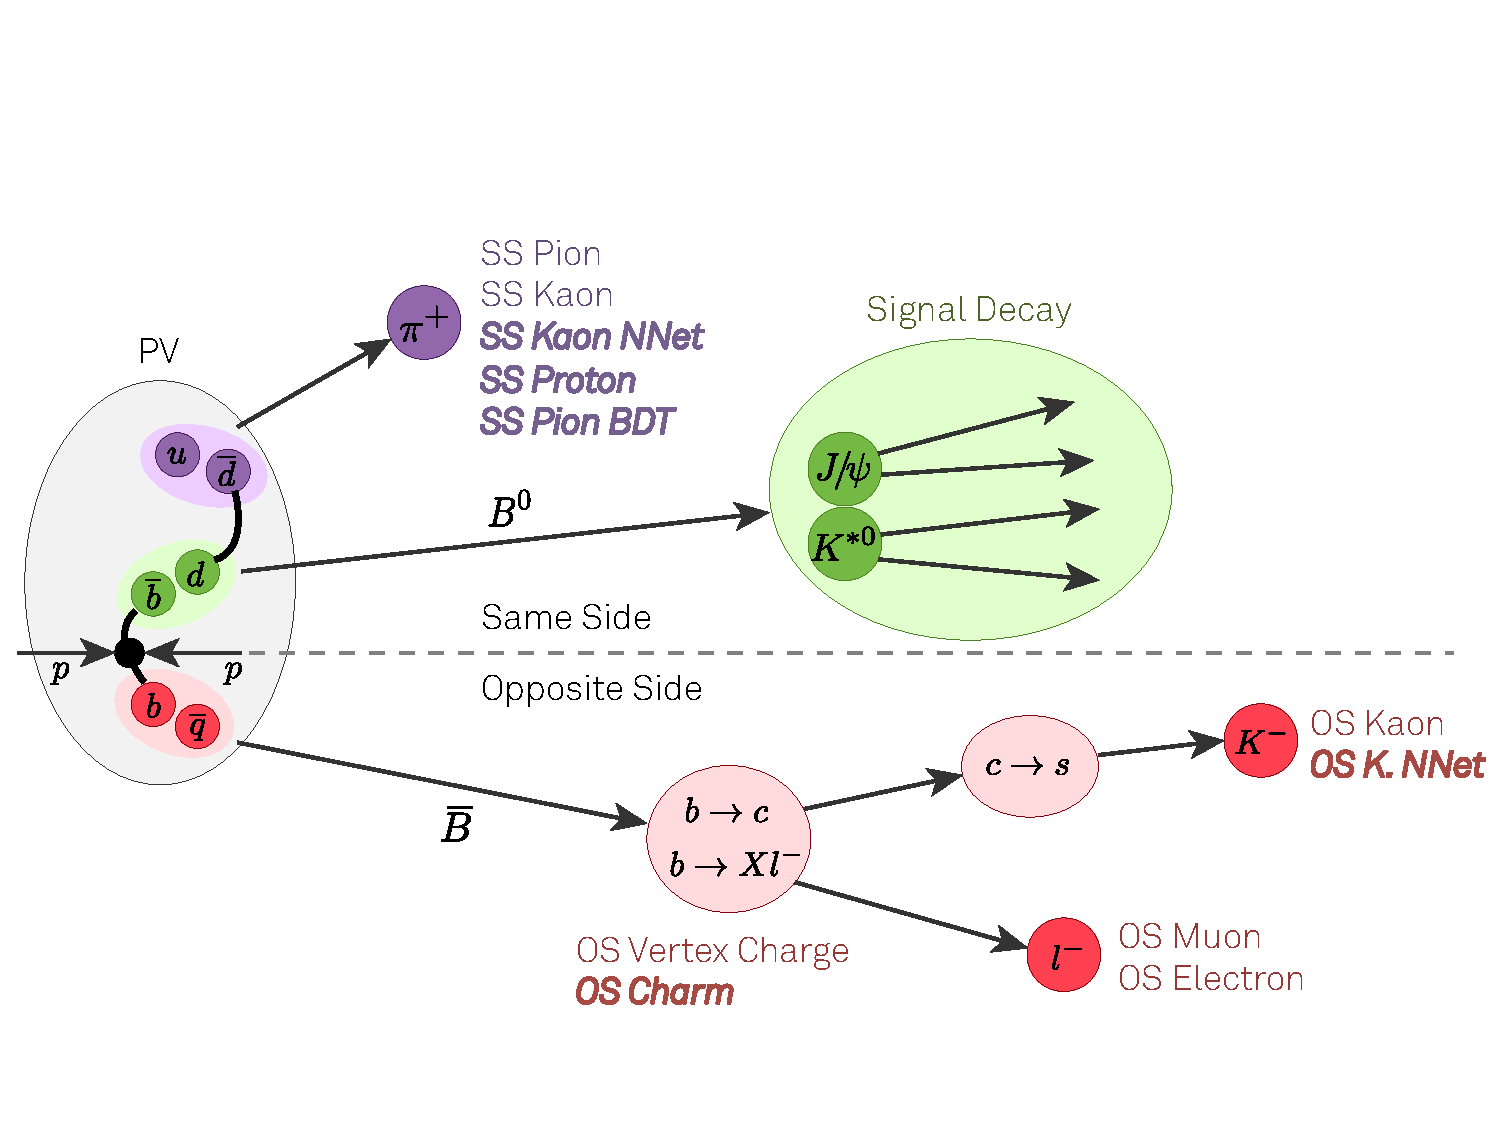
\includegraphics[width=\textwidth]{images/FlavourTaggingScheme.pdf}
    \caption{Schematic overview of the underlying principles of LHCb's flavour tagging algorithms \cite{ft_scheme}.}
    \label{fig:ft_scheme}
\end{figure}

When a $B$ meson in a $pp$-collision is Lorentz boosted, it is possible to distinguish its production point from its decay point.
This allows matching the decay particles to the signal $B$.
The production point, i.e. the collision point of the $pp$ pair, is called the primary vertex~(PV) and the decay point is called the secondary vertex~(SV).
Identifying the type of signal $B$ can be done by reconstructing either the signal decay or the associated event. 
The latter method is independent of the signal decay channel, and it is often used in flavour tagging algorithms at LHCb. 
A similar method is used in this thesis.
% TODO: clear separation between flavour tagging and the topic of this thesis

The back-to-back production in the rest frame of the $b\bar{b}$ pair leads to an angular separation of the associated event into two \enquote{sides}.
The \enquote{same side}~(SS) contains the decay particles and the fragmentation particles of the signal $B$.
The \enquote{opposite side}~(OS) contains all particles associated with the $b$ quark that is not in the signal $B$.
For the distinction between $B_d$ and $B_s$ mesons, it is irrelevant if the signal $B$ contains a $b$ quark or an $\bar{b}$ quark.
Therefore, it is expected that only the SS fragmentation contains relevant information for this thesis.
% TODO: transition to the classification algorithms chapter
